\documentclass[border=2pt]{standalone}
\usepackage{tikz}
\usetikzlibrary{arrows.meta,positioning}
\usepackage{mathptmx}
\begin{document}

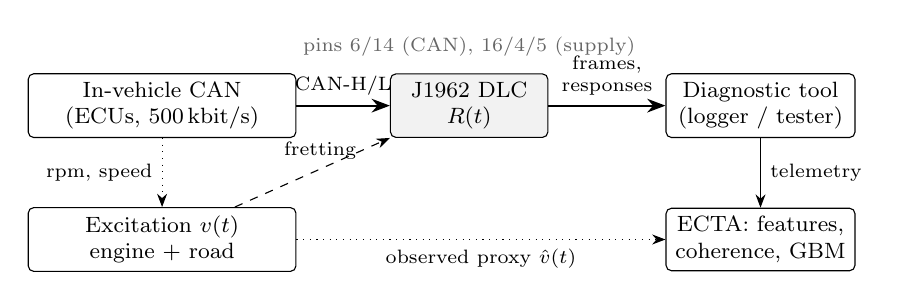
\begin{tikzpicture}[font=\footnotesize, >=Stealth,
  box/.style={draw, rounded corners=2pt, align=center, minimum height=7mm, inner sep=3pt},
  lab/.style={align=center, font=\scriptsize}]
\node[box, minimum width=34mm] (bus) at (0,0) {In-vehicle CAN\\(ECUs, 500\,kbit/s)};
\node[box, minimum width=20mm, fill=black!5] (dlc) at (3.9,0) {J1962 DLC\\$R(t)$};
\node[box, minimum width=24mm] (tool) at (7.6,0) {Diagnostic tool\\(logger / tester)};
\node[box, minimum width=24mm] (ecta) at (7.6,-1.7) {ECTA: features,\\coherence, GBM};
\node[box, minimum width=34mm] (exc) at (0,-1.7) {Excitation $v(t)$\\engine + road};
\draw[->, thick] (bus) -- node[above, lab]{CAN-H/L}(dlc);
\draw[->, thick] (dlc) -- node[above, lab]{frames,\\responses}(tool);
\draw[->] (tool) -- node[right, lab]{telemetry}(ecta);
\draw[->, dashed] (exc) -- node[above, lab, pos=0.55]{fretting}(dlc.south west);
\draw[->, dotted] (bus.south) -- node[left, lab]{rpm, speed}(exc.north);
\draw[->, dotted] (exc.east) -- node[below, lab]{observed proxy $\hat v(t)$}(ecta.west);
\node[lab, text=black!60] at (3.9,0.75) {pins 6/14 (CAN), 16/4/5 (supply)};
\end{tikzpicture}
\end{document}
